\section{The overlap, and the probabilistic call}
\label{sec:decision}

\begin{figure*}[t]
\centering
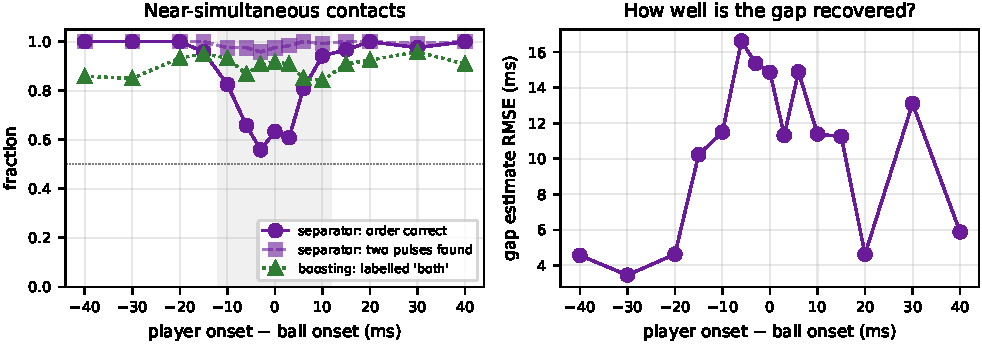
\includegraphics[width=\textwidth]{figures/overlap.pdf}
\caption{The anomalous case: ball and player struck within one window, versus
the signed gap (player onset minus ball onset; negative = player first). Left:
the separator finds two pulses almost always and orders them correctly outside
the shaded band (one ball-pulse duration), while the boosting classifier
labels the window \emph{both} at a roughly constant rate regardless of gap.
Right: RMSE of the recovered gap.}
\label{fig:overlap}
\end{figure*}

\paragraph{The anomalous overlap.} Figure~\ref{fig:overlap} maps the case the
project was started for: the boot hits the opponent and the ball inside one
pulse width. With \OvlNPerGap\ windows per gap at \OvlFs\,Hz, the two-template
separator declares two pulses in at least \OvlTwoMin\ of windows at every gap,
and orders them correctly in \OvlAccTwenty\ of cases at $\pm20$\,ms,
\OvlAccFifteen\ at $\pm15$\,ms, \OvlAccTen\ at $\pm10$\,ms, \OvlAccSix\ at
$\pm6$\,ms and \OvlAccThree\ at $\pm3$\,ms (\OvlAccZero\ at zero, which is
chance by construction). The gap itself is recovered to \OvlGapRmseWide\,ms
RMSE when the pulses are 20\,ms or more apart and only to
\OvlGapRmseNarrow\,ms inside the overlap. The boosting classifier, by contrast,
labels \OvlGbBothMin--\OvlGbBothMax\ of these windows \emph{both} at every gap:
it knows two things were hit but has no notion of order. The shape of the
left panel is the physical content of this paper: the ball pulse lasts
7--12\,ms, so two contacts closer than that share their rising edges and no
estimator can tell which began first from the boot alone. Above about one
pulse duration the order is recoverable and above two it is essentially
certain.

\begin{figure*}[t]
\centering
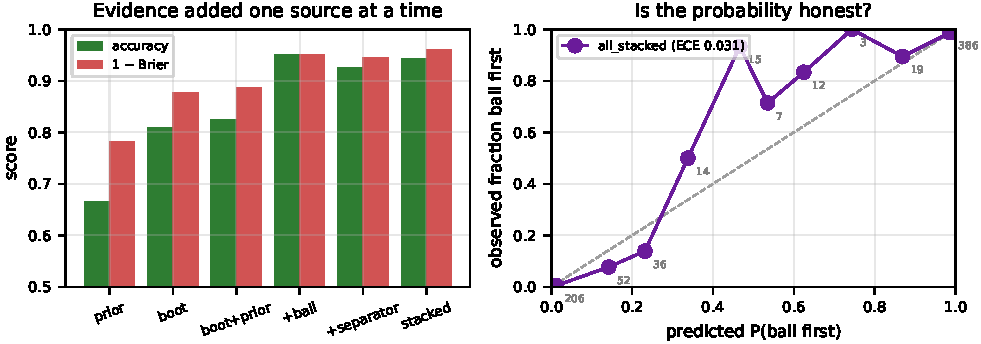
\includegraphics[width=\textwidth]{figures/decision.pdf}
\caption{Left: accuracy and $1-$Brier of $P(\text{ball first})$ as evidence is
added --- knowledge-base prior, boot classifier, ball-sensor timing, separator
order --- with naive-Bayes fusion, and the stacked logistic fusion of all
sources. Right: reliability diagram of the best model (bin counts in grey).}
\label{fig:decision}
\end{figure*}

\paragraph{From evidence to a probability.} Figure~\ref{fig:decision} reports
the decision layer on \DecNEval\ held-out challenges (half clean single
contacts, half overlaps with gaps of 2--40\,ms; base rate of ball-first
\DecBaseRate). The knowledge-base prior alone is right \DecPriorAcc\ of the
time with Brier \DecPriorBrier: base rates are informative but not decisive.
The boot classifier alone reaches \DecBootAcc\ --- essentially perfect on
clean contacts (\DecBootAccSingle) and near chance on overlaps
(\DecBootAccBoth), for the reason just given. Adding the ball sensor's timing
is the step that matters: accuracy \DecBootBallAcc, Brier \DecBootBallBrier,
with overlaps now at \DecBootBallAccBoth. Adding the separator's order under
naive-Bayes fusion \emph{hurts} slightly (\DecAllAcc), because the boot
posterior and the separator read the same window and are double-counted; the
stacked logistic fusion resolves this (accuracy \DecStackAcc, Brier
\DecStackBrier, ECE \DecStackEce), learning weights of \DecCoefBoot\ (boot),
\DecCoefBall\ (ball timing), \DecCoefSep\ (separator) and \DecCoefPrior\
(prior) on the calibrated log-odds. The reliability diagram shows the
probabilities are honest across the range; the situation where the prior is
most wrong (a late challenge, prior \DecLateAccPrior\ accuracy) is where the
sensors help most (\DecLateAccAll).

\paragraph{The call.} With equal costs for a false foul and a missed foul the
threshold is $0.5$ and the error rate is \DecErrNoReview\%; adding a review
band of $\pm0.15$ refers \DecReviewRate\% of challenges to video and lowers the
error among those decided on the field to \DecErrDecided\%. If a false foul is
judged four times as costly as a missed one, the threshold moves to
\DecThrFour\ and false fouls fall from \DecFalseFoulOne\% to
\DecFalseFoulFour\% of challenges while missed fouls rise from
\DecMissedOne\% to \DecMissedFour\%. The point of a calibrated probability is
exactly that this trade is a policy setting, not a retraining.
